\documentclass{beamer}
\usepackage[utf8]{inputenc}
\usepackage[german]{babel}
\usepackage{graphicx}
\usepackage{tikz}
\usepackage{xcolor}
\usepackage[export]{adjustbox}
\usepackage{subfig}
\usepackage{graphbox}
\usepackage[autostyle=true,german=quotes]{csquotes}

\MakeOuterQuote{"}

\begin{document}

\title{\fontsize{60}{60} \selectfont GO}
\author{Hugo Platzer}
\subtitle{Eine Einführung in das asiatische Brettspiel}
\date{}

\setbeamertemplate{navigation symbols}{}
\addtobeamertemplate{navigation symbols}{}{
    \usebeamerfont{footline}
    \usebeamercolor[fg]{footline}
    \hspace{1em}
    \insertframenumber/\inserttotalframenumber
}

{
\setbeamertemplate{headline}{\vskip\headheight}
\setbeamertemplate{footline}{}
\usebackgroundtemplate{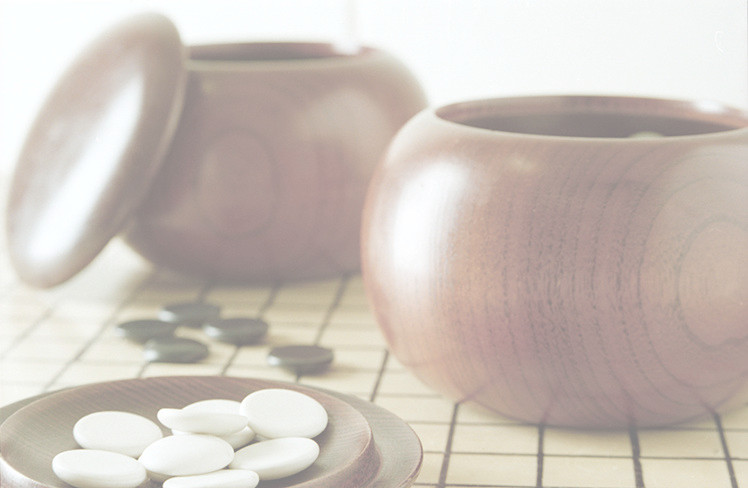
\includegraphics[width=\paperwidth,height=\paperheight]{images/bowls_board_faded.jpg}}
\frame{\titlepage}
}

\frame{\frametitle{Was ist Go?}
  \begin{itemize}
    \item Brettspiel für 2 Personen (Schwarz vs. Weiß)
    \item vor min. 2500 Jahren im antiken China erfunden
    \item Spielbrett: quadratisches Gitter, auf Schnittpunkte werden Steine gesetzt
    \item Ziel: am Ende mehr als die Hälfte des Bretts zu besitzen
  \end{itemize}
  \vspace{0.1cm}
  \noindent\makebox[\textwidth]{
  \hspace{-1cm}
  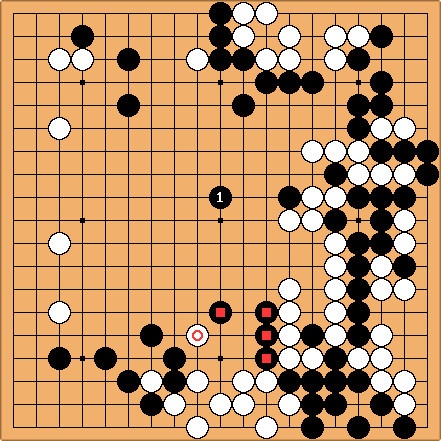
\includegraphics[height=4.5cm]{images/go_example.jpg}
  }
}

\frame{\frametitle{Spielregeln}
  \begin{enumerate}
    \item Spieler machen abwechselnd einen Zug (Schwarz beginnt)
    \item Zug: Setzen oder passen (nichts tun, Gegner an der Reihe)
    \item Setzen: Stein auf freien Punkt, zuerst gegnerische Ketten entfernen,
          dann eigene Ketten entfernen
    \item Kette wird entfernt, falls sie keine Freiheiten hat
    \item Freiheiten einer Kette: freie Punkte, die $\leftrightarrow \updownarrow$ an einen Stein der Kette
           angrenzen
    \item Setzen nicht erlaubt, falls es zu Zyklus führt
    \item beide Spieler passen hintereinander $\Rightarrow$ Auszählung
    \item Punkte pro Spieler: Anzahl Steine am Brett plus Gebiet
    \item Gebiet eines Spielers: freie Punkte, von denen man via $\leftrightarrow \updownarrow$  zur
          Farbe des Spielers kommt, nicht aber zur gegnerischen
    \item Spieler mit mehr Punkten gewinnt
  \end{enumerate}
}

\frame{\frametitle{Spielregeln erklärt}
\centering
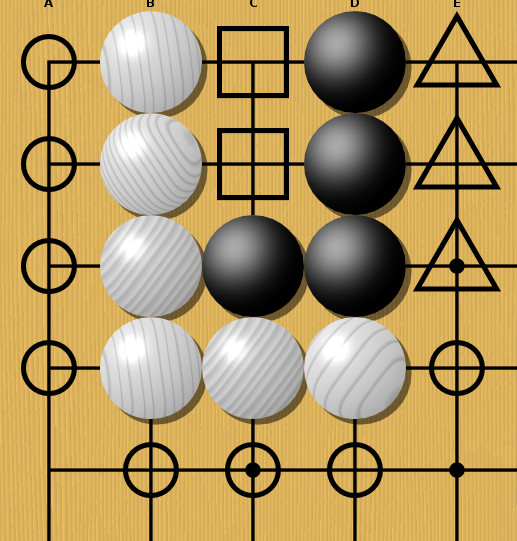
\includegraphics[height=4cm]{images/rules_liberty.jpg}
\captionof{figure}{Freiheiten}

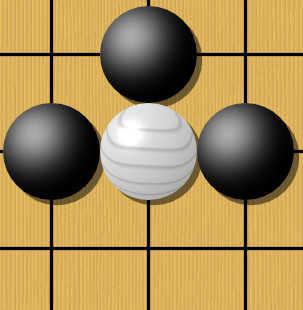
\includegraphics[height=3cm]{images/rules_capture1.jpg}
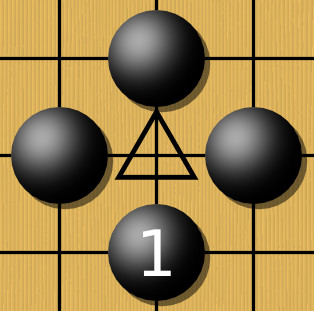
\includegraphics[height=3cm]{images/rules_capture2.jpg}
\captionof{figure}{Schlagen 1}
}

\frame{\frametitle{Spielregeln erklärt}
\centering
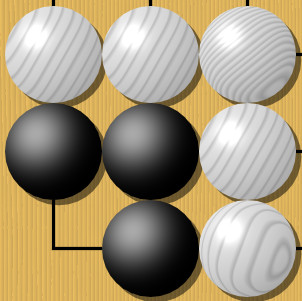
\includegraphics[height=3cm]{images/rules_capture3.jpg}
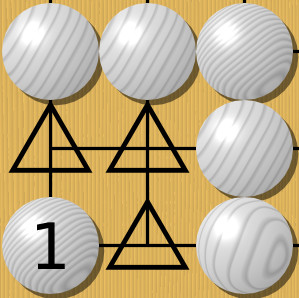
\includegraphics[height=3cm]{images/rules_capture4.jpg}
\captionof{figure}{Schlagen 2}

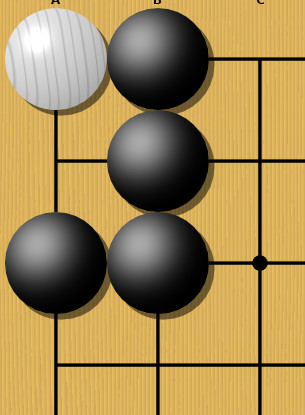
\includegraphics[height=3cm]{images/rules_suicide1.jpg}
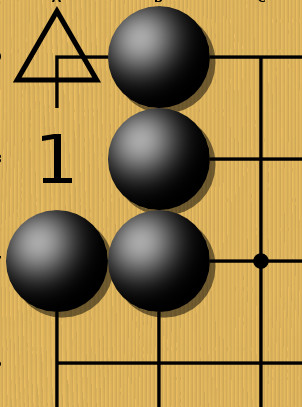
\includegraphics[height=3cm]{images/rules_suicide2.jpg}
\captionof{figure}{Selbstmord}
}

\frame{\frametitle{Spielregeln erklärt}
\centering
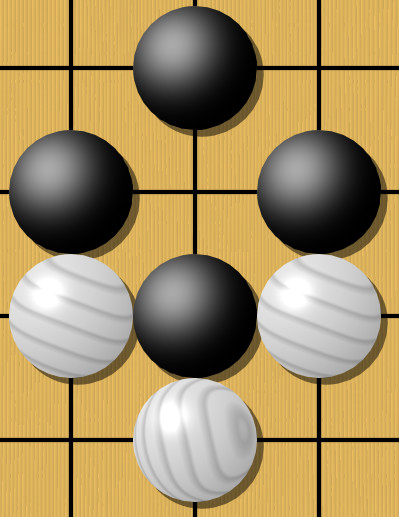
\includegraphics[height=2.5cm]{images/rules_ko1.jpg}
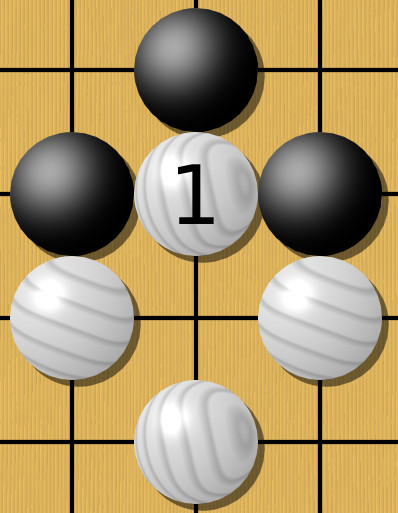
\includegraphics[height=2.5cm]{images/rules_ko2.jpg}
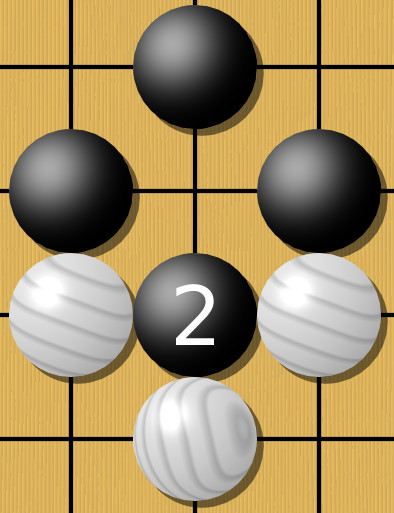
\includegraphics[height=2.5cm]{images/rules_ko3.jpg}
\captionof{figure}{Zyklus (Ko)}

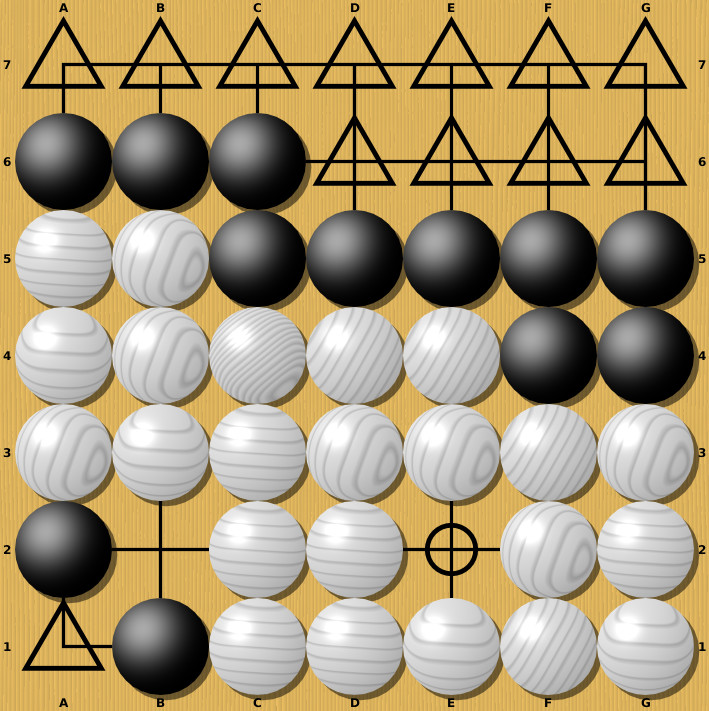
\includegraphics[height=4cm]{images/rules_scoring.jpg}
\captionof{figure}{Auszählung}
}

\frame{\frametitle{Taktiken / Motive}
\centering
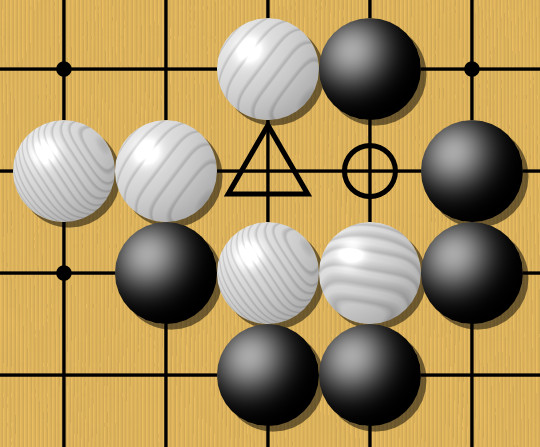
\includegraphics[height=3cm]{images/tactic_snapback.jpg}
\captionof{figure}{Mausefalle}

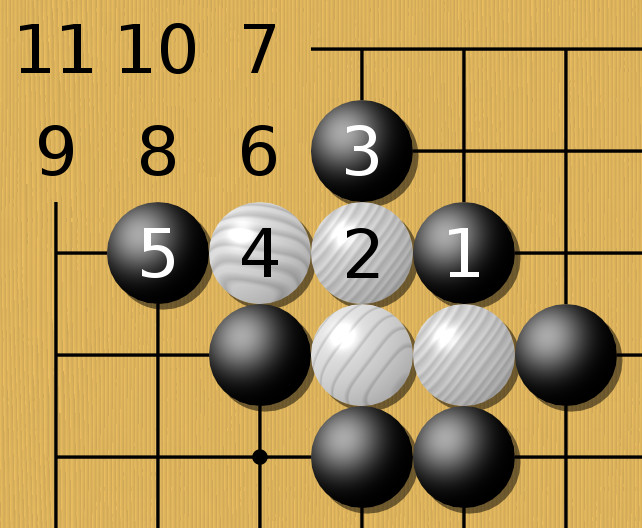
\includegraphics[height=3cm]{images/tactic_ladder.jpg}
\captionof{figure}{Treppe}
}

\frame{\frametitle{Taktiken / Motive}
\centering
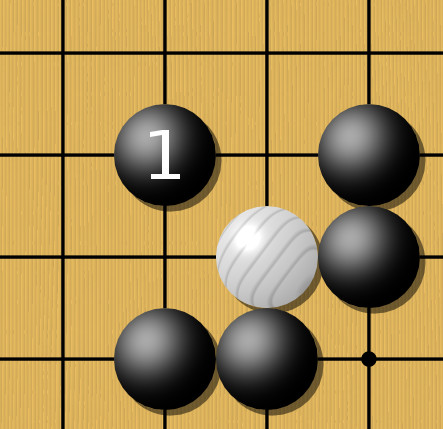
\includegraphics[height=3cm]{images/tactic_net.jpg}
\captionof{figure}{Netz}

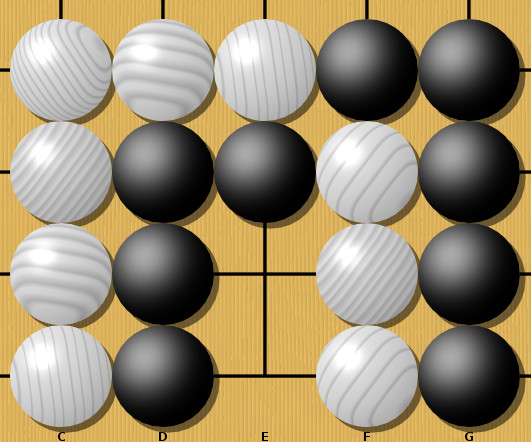
\includegraphics[height=3cm]{images/tactic_seki.jpg}
\captionof{figure}{Seki}
}

\frame{\frametitle{Leben und Tod}
\centering
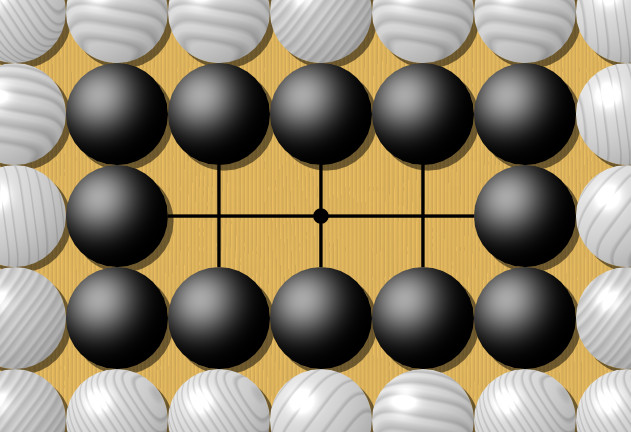
\includegraphics[height=3cm]{images/lnd_1.jpg}
\hspace{0.5cm}
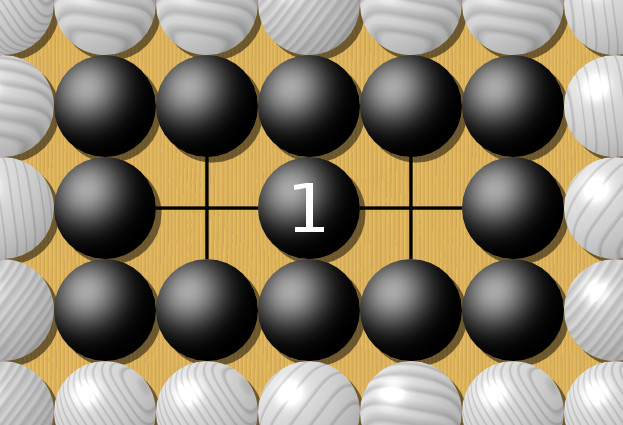
\includegraphics[height=3cm]{images/lnd_2.jpg}

\vspace{0.5cm}
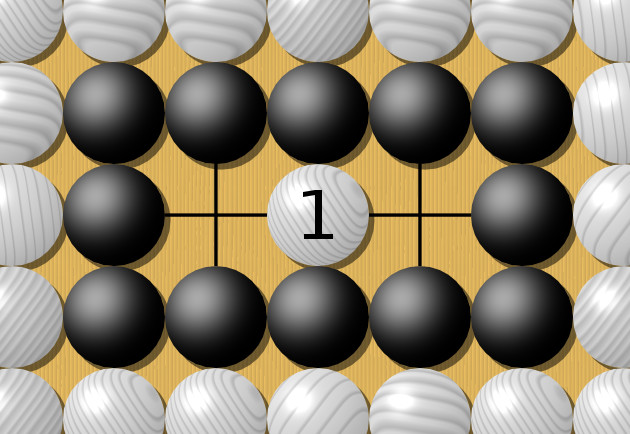
\includegraphics[height=3cm]{images/lnd_3.jpg}
\hspace{0.5cm}
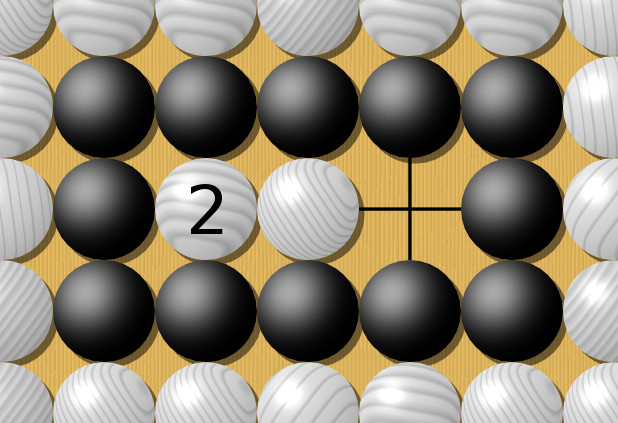
\includegraphics[height=3cm]{images/lnd_4.jpg}
}

\frame{\frametitle{Leben und Tod}
\centering
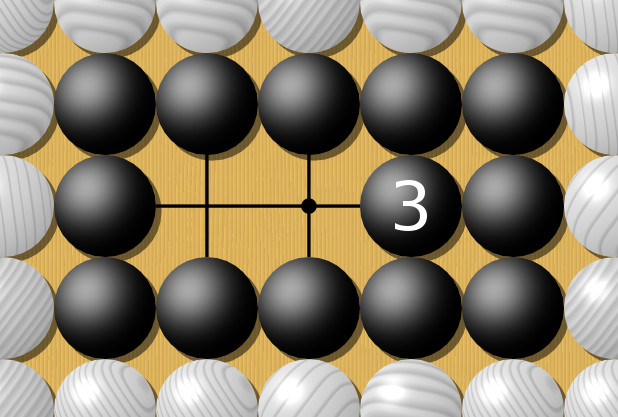
\includegraphics[height=3cm]{images/lnd_5.jpg}
\hspace{0.5cm}
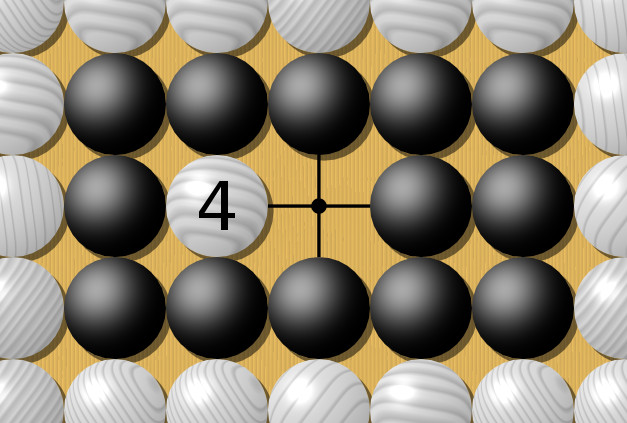
\includegraphics[height=3cm]{images/lnd_6.jpg}

\vspace{0.5cm}
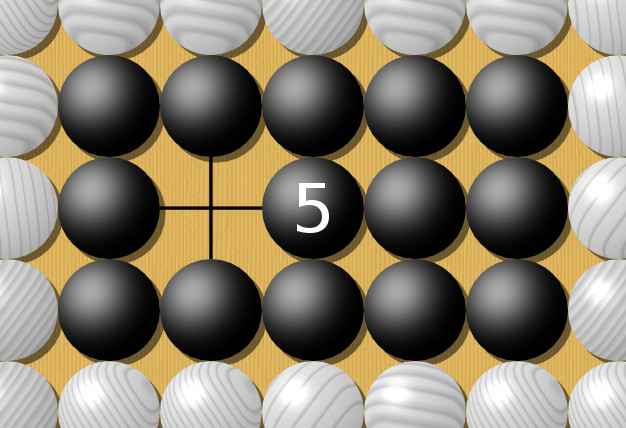
\includegraphics[height=3cm]{images/lnd_7.jpg}
\hspace{0.5cm}
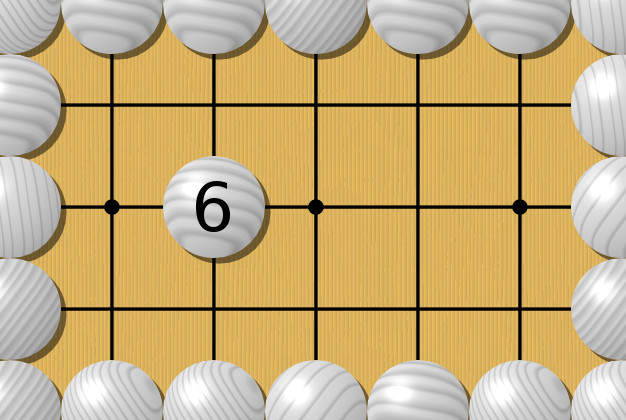
\includegraphics[height=3cm]{images/lnd_8.jpg}
}

\frame{\frametitle{Formen}
\centering
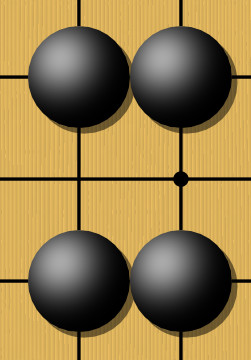
\includegraphics[height=2.5cm]{images/shape_bamboojoint.jpg} \hspace{2cm}
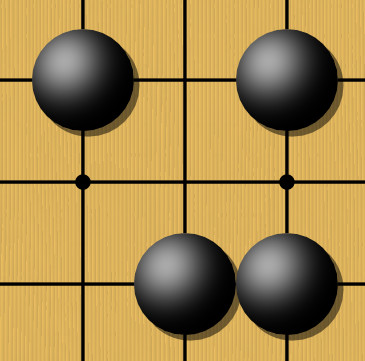
\includegraphics[height=2.5cm]{images/shape_table.jpg}
\captionof{figure}{Bambus, Tisch}

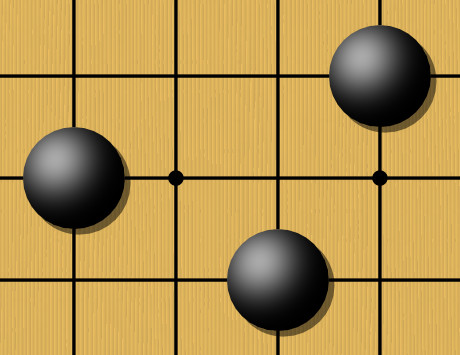
\includegraphics[height=2.5cm]{images/shape_bumerang.jpg} \hspace{2cm}
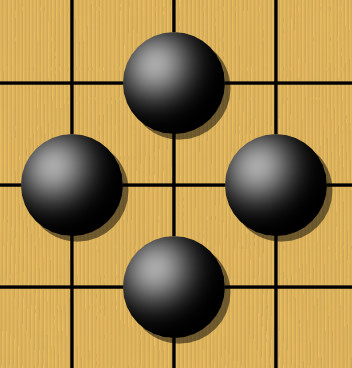
\includegraphics[height=2.5cm]{images/shape_ponnuki.jpg}
\captionof{figure}{Bumerang, Todesstern}
}

\frame{\frametitle{Strategie}
  \begin{itemize}
    \item durch Kenntnisse über Leben und Tod wissen Spieler oft schon früh,
          dass Gebiet sicher ist
    \item Eigene Steine verbinden, gegnerische trennen (schneiden)
    \item nicht in einzelnen Steinen, sondern in Regionen des Bretts denken
    \item Tauschhandel mit dem Gegner, man kann nicht alles haben $\rightarrow$ Kompromissbereitschaft!
    \item Genügsamkeit vs Gier (man braucht nur einen Punkt mehr)
    \item Zentrum vs Ecke / Ränder
  \end{itemize}
}

\frame{\frametitle{Bezug zur Informatik}
  \begin{itemize}
    \item AlphaGo
  \end{itemize}
}

\frame{\frametitle{Bezug zur Informatik}
  \begin{itemize}
    \item Minmax
  \end{itemize}
}

\frame{\frametitle{Spielstärke / Handicap}
  \begin{itemize}
    \item Go-Spieler werden (von Servern, Spielergemeinschaften etc.)
          nach Spielstärke bewertet (30 kyu - 1 kyu, 1 dan - 9 dan)
    \item Go hat Mechanismus, um Gewinnchancen bei ungleich starken
          Spielern gleich zu halten
    \item schwächerer Spieer platziert vor Spielstart mehrere Steine auf
          bestimmte Punkte
          
    \vspace{0.3cm}
    \noindent\makebox[\textwidth]{
    \hspace{-8cm}
    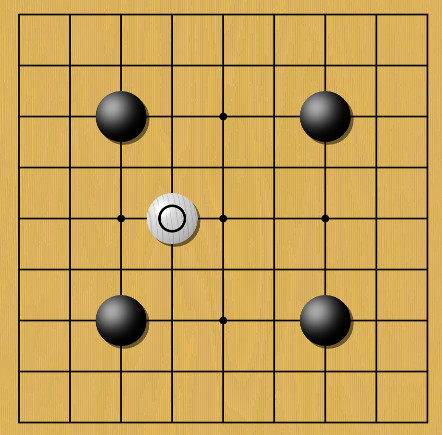
\includegraphics[width=3cm]{images/handicap.jpg}
    }
    
    \item 1 Stein Handicap - 1 Rang Unterschied
  \end{itemize}
}

\frame{\frametitle{Vergleich zu anderen Brettspielen}
    \noindent\makebox[\textwidth]{
    \centering
    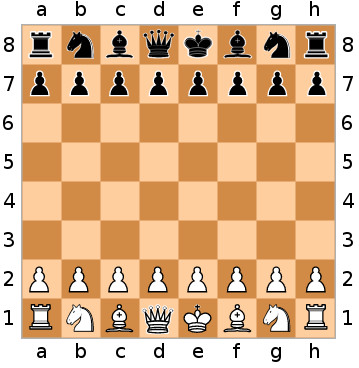
\includegraphics[height=3cm, width=3cm]{images/other_chess.jpg}
    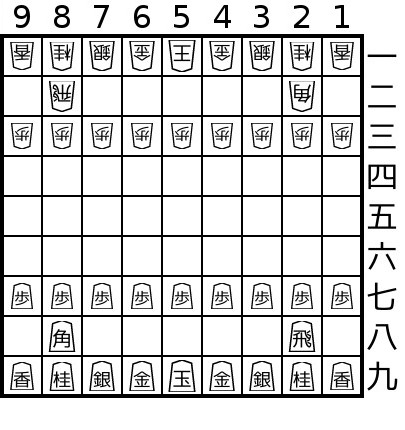
\includegraphics[height=3cm, width=3cm]{images/other_shogi.jpg}
    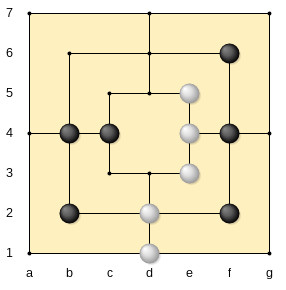
\includegraphics[height=3cm, width=3cm]{images/other_morris.jpg}
    }
  \begin{itemize}
    \item keine unterschiedlichen Spielfiguren: der Wert eines Steins definiert sich einzig durch seine Beziehung zu anderen Steinen!
    \item größeres Spielbrett, mehr mögliche Züge / Brettstellungen
    \item kein Remis (je nach Regelvariante)
    \item Punktewertung: jeder Punkt ist gleich viel wert, kein einzelnes Ziel (König)
    \item größerer Fokus auf Intuition, diffuses / langfristiges Planen
          anstatt konkrete Taktiken
  \end{itemize}
}

\frame{\frametitle{Warum sollte man Go (nicht) spielen?}
  {\bf Pro:}
  \begin{itemize}
    \item Regeln einfach, aber man lernt nie aus
    \item viel mögliche Abwechslung bei Strategien
    \item abstrakte virtuelle Realität: bildet die Welt ab
    \item Lektionen fürs Leben: diszipliniert lernen, mit Verlusten umgehen
    \item lange Tradition, viele Spieler auf der ganzen Welt
    \item Computer
  \end{itemize}
  
  {\bf Contra:}
  \begin{itemize}
    \item steile Lernkurve, besonders am Anfang, Stagnation
    \item großer Zeitaufwand
    \item sehr hierarchisch (Ränge)
    \item Computer
  \end{itemize} 
}



\end{document}
